\begin{abstract}
In January and August of 2014, two unusual transient events were observed in a strongly lensed galaxy at z=1.0054$\pm$0.0002.  
Discovered by the FrontierSN team in Hubble Space Telescope (HST) observations from the Hubble Frontier Fields (HFF) program, these events are designated HFF14Spo-SE and HFF14Spo-NW, and collectively nicknamed ``Spock''.  Both transient episodes  were faster and fainter than any normal supernova: they rose to a peak absolute optical/ultraviolet luminosity of $M\sim-14$ mag ($10^{40}$ ergs/sec) in only $\sim$3 rest-frame days, and then faded away below detectability in roughly the same amount of time.  These events appeared in two adjacent arcs of a strongly lensed galaxy that is multiply-imaged into at least 3 distinct images by the gravitational potential of the galaxy cluster MACSJ0416 (z=0.396).  Using four independent lens models of this cluster, we find it is entirely plausible that the NW and SE events are {\it spatially} coincident on the source plane, but very unlikely that they were also {\it temporally} coincident.  We evaluate several physical models for these events, and find that the least disfavored explanation is that we have observed two distinct outbursts from a single extraordinary recurrent nova.  This model would imply that the HFF14Spo system has the fastest known recurrence timescale of any nova ($\sim$8 months).  Further, if our estimate for the gravitational lensing magnification is correct, then HFF14Spo is about 2 orders of magnitude more luminous than an average nova.  This model would therefore require that the HFF14Spo system's primary star is a white dwarf very close to the Chandrasekhar mass limit, and that it is drawing mass from the secondary at an extremely efficient rate (??? $>10^{-8}$ \Msun/yr ???).  This in turn suggests that this system is a strong candidate to eventually explode as a Type Ia Supernova. 
\end{abstract}

\section{Introduction}\label{sec:Introduction}

\section{Observations}\label{sec:Observations}

\subsection{Host Galaxy Spectroscopy}\label{sec:HostGalaxySpectroscopy}

\begin{figure}
\begin{center}
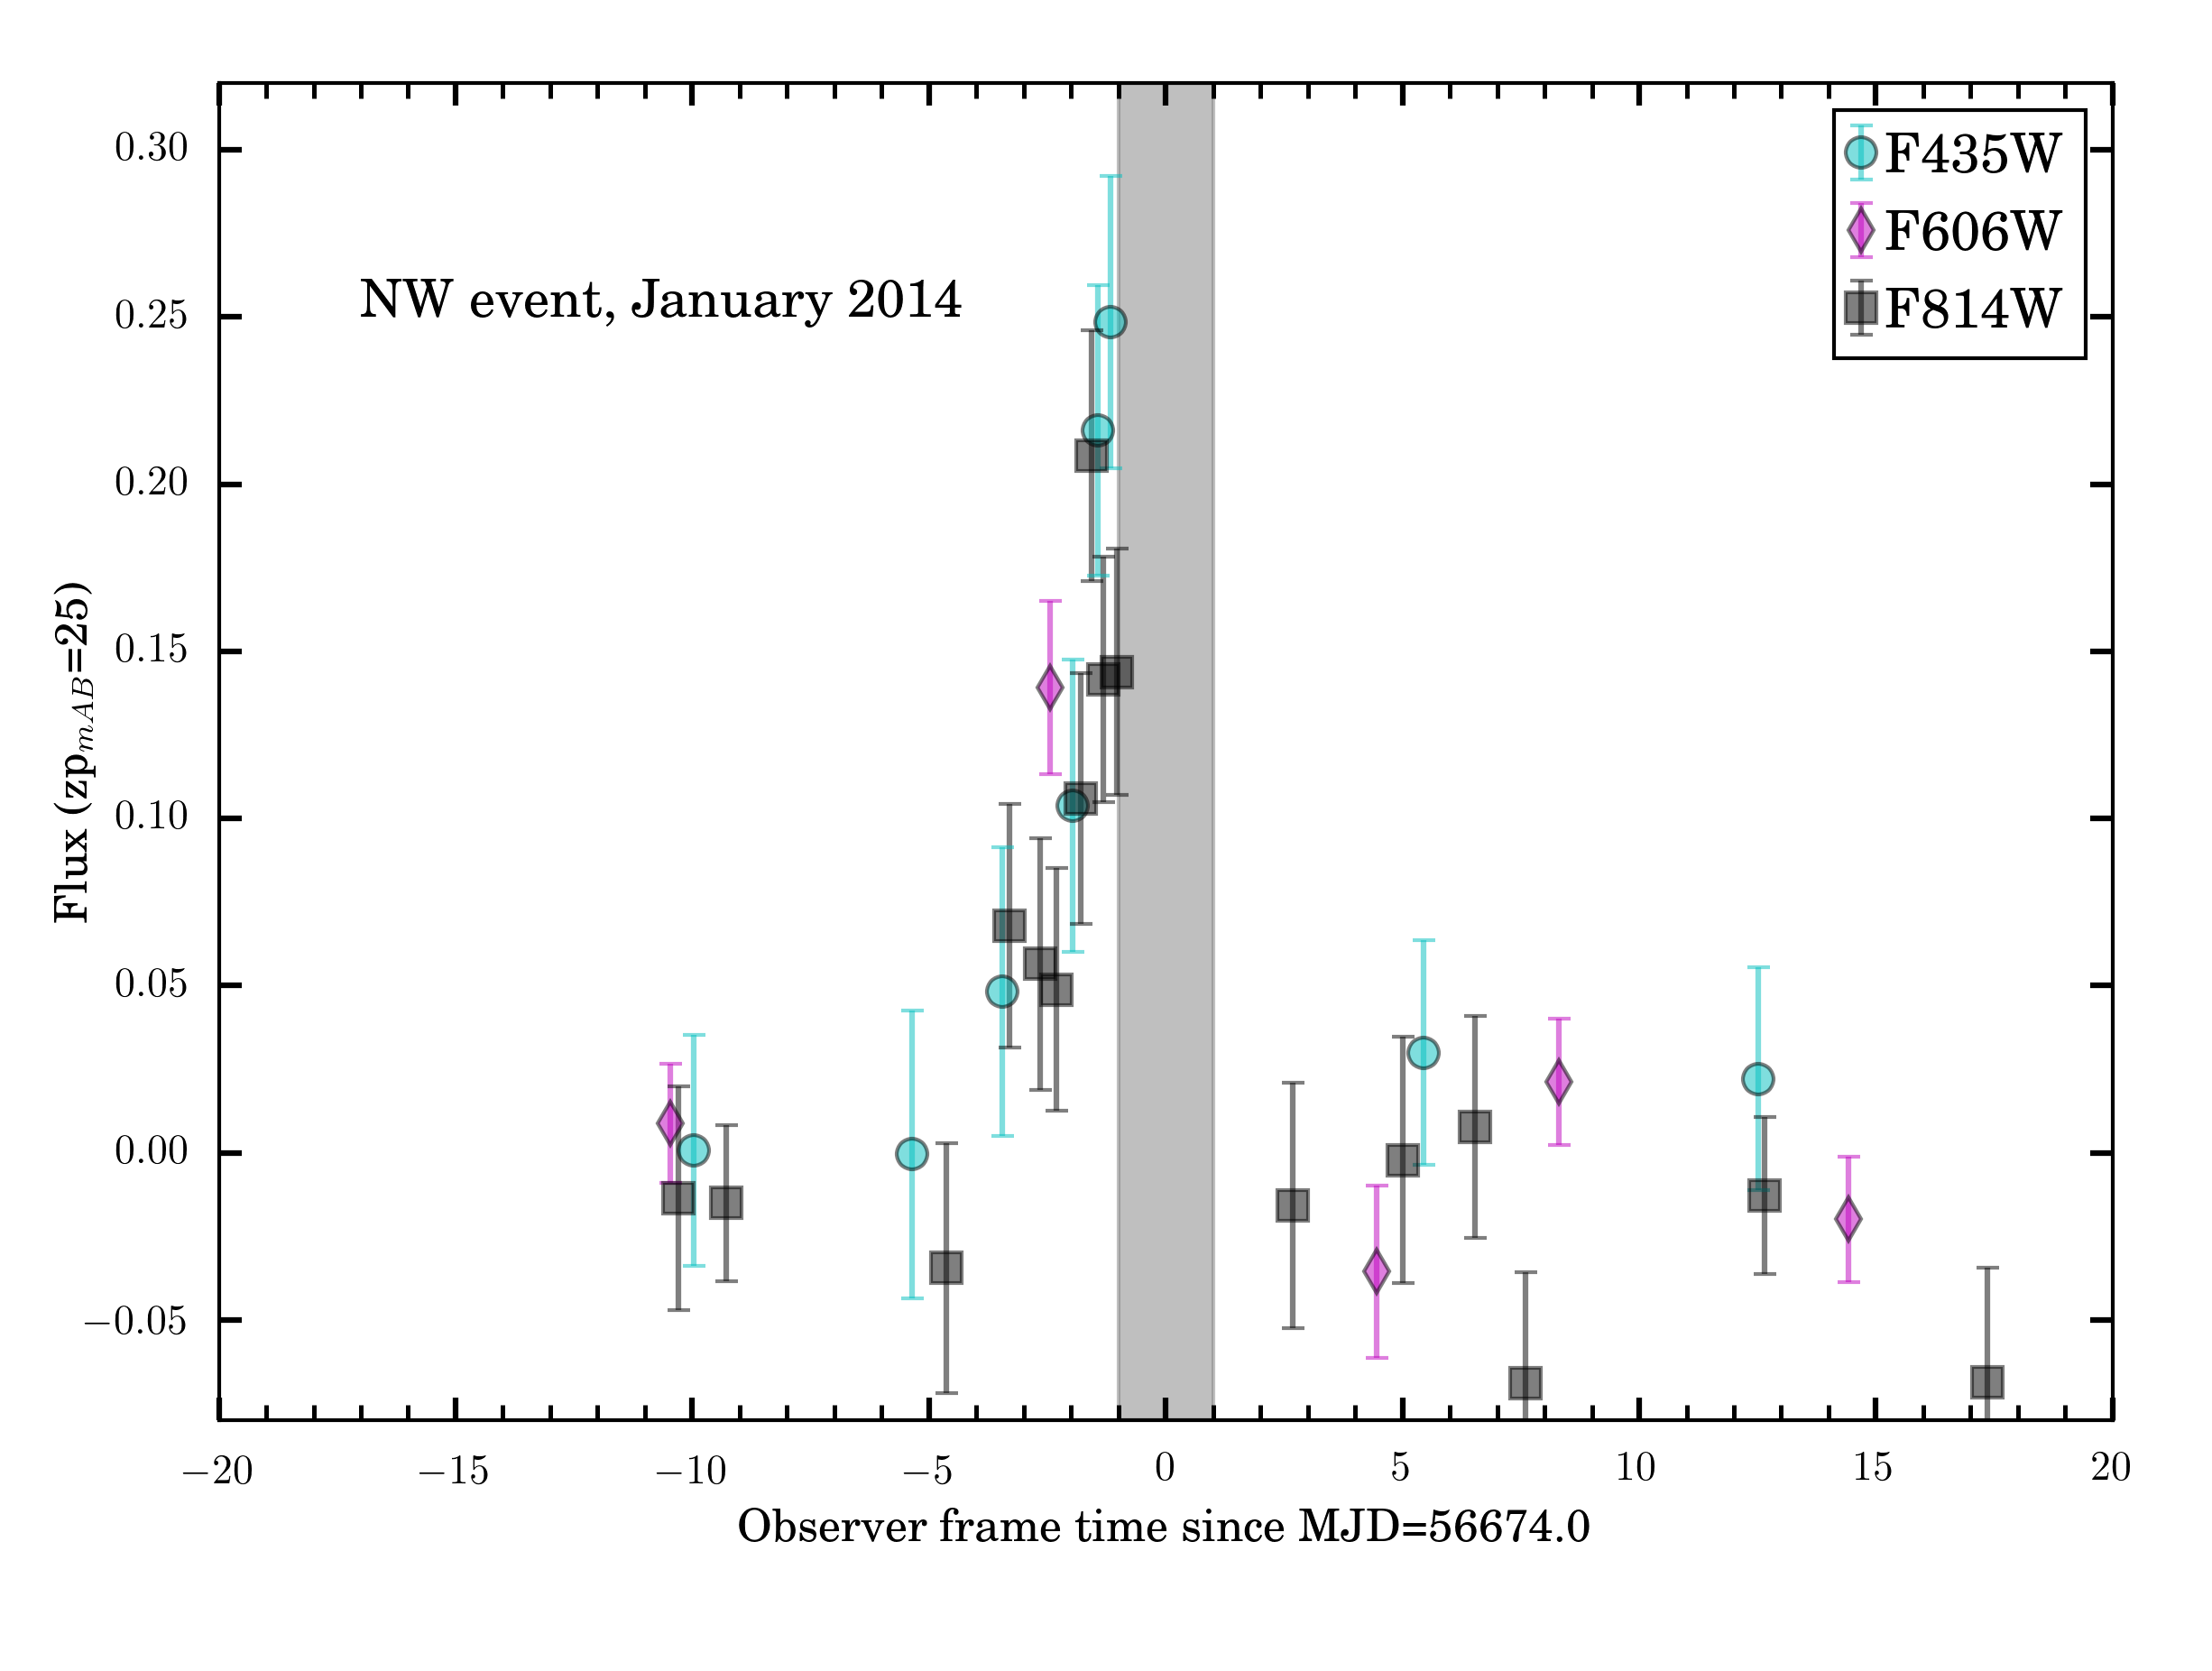
\includegraphics[width=\columnwidth]{figures/m0416_transient_NW.png}
\caption{The light curve of the January 2014 transient event, HFF14Spo-NW.}
\end{center}
\end{figure}


\begin{figure}
\begin{center}
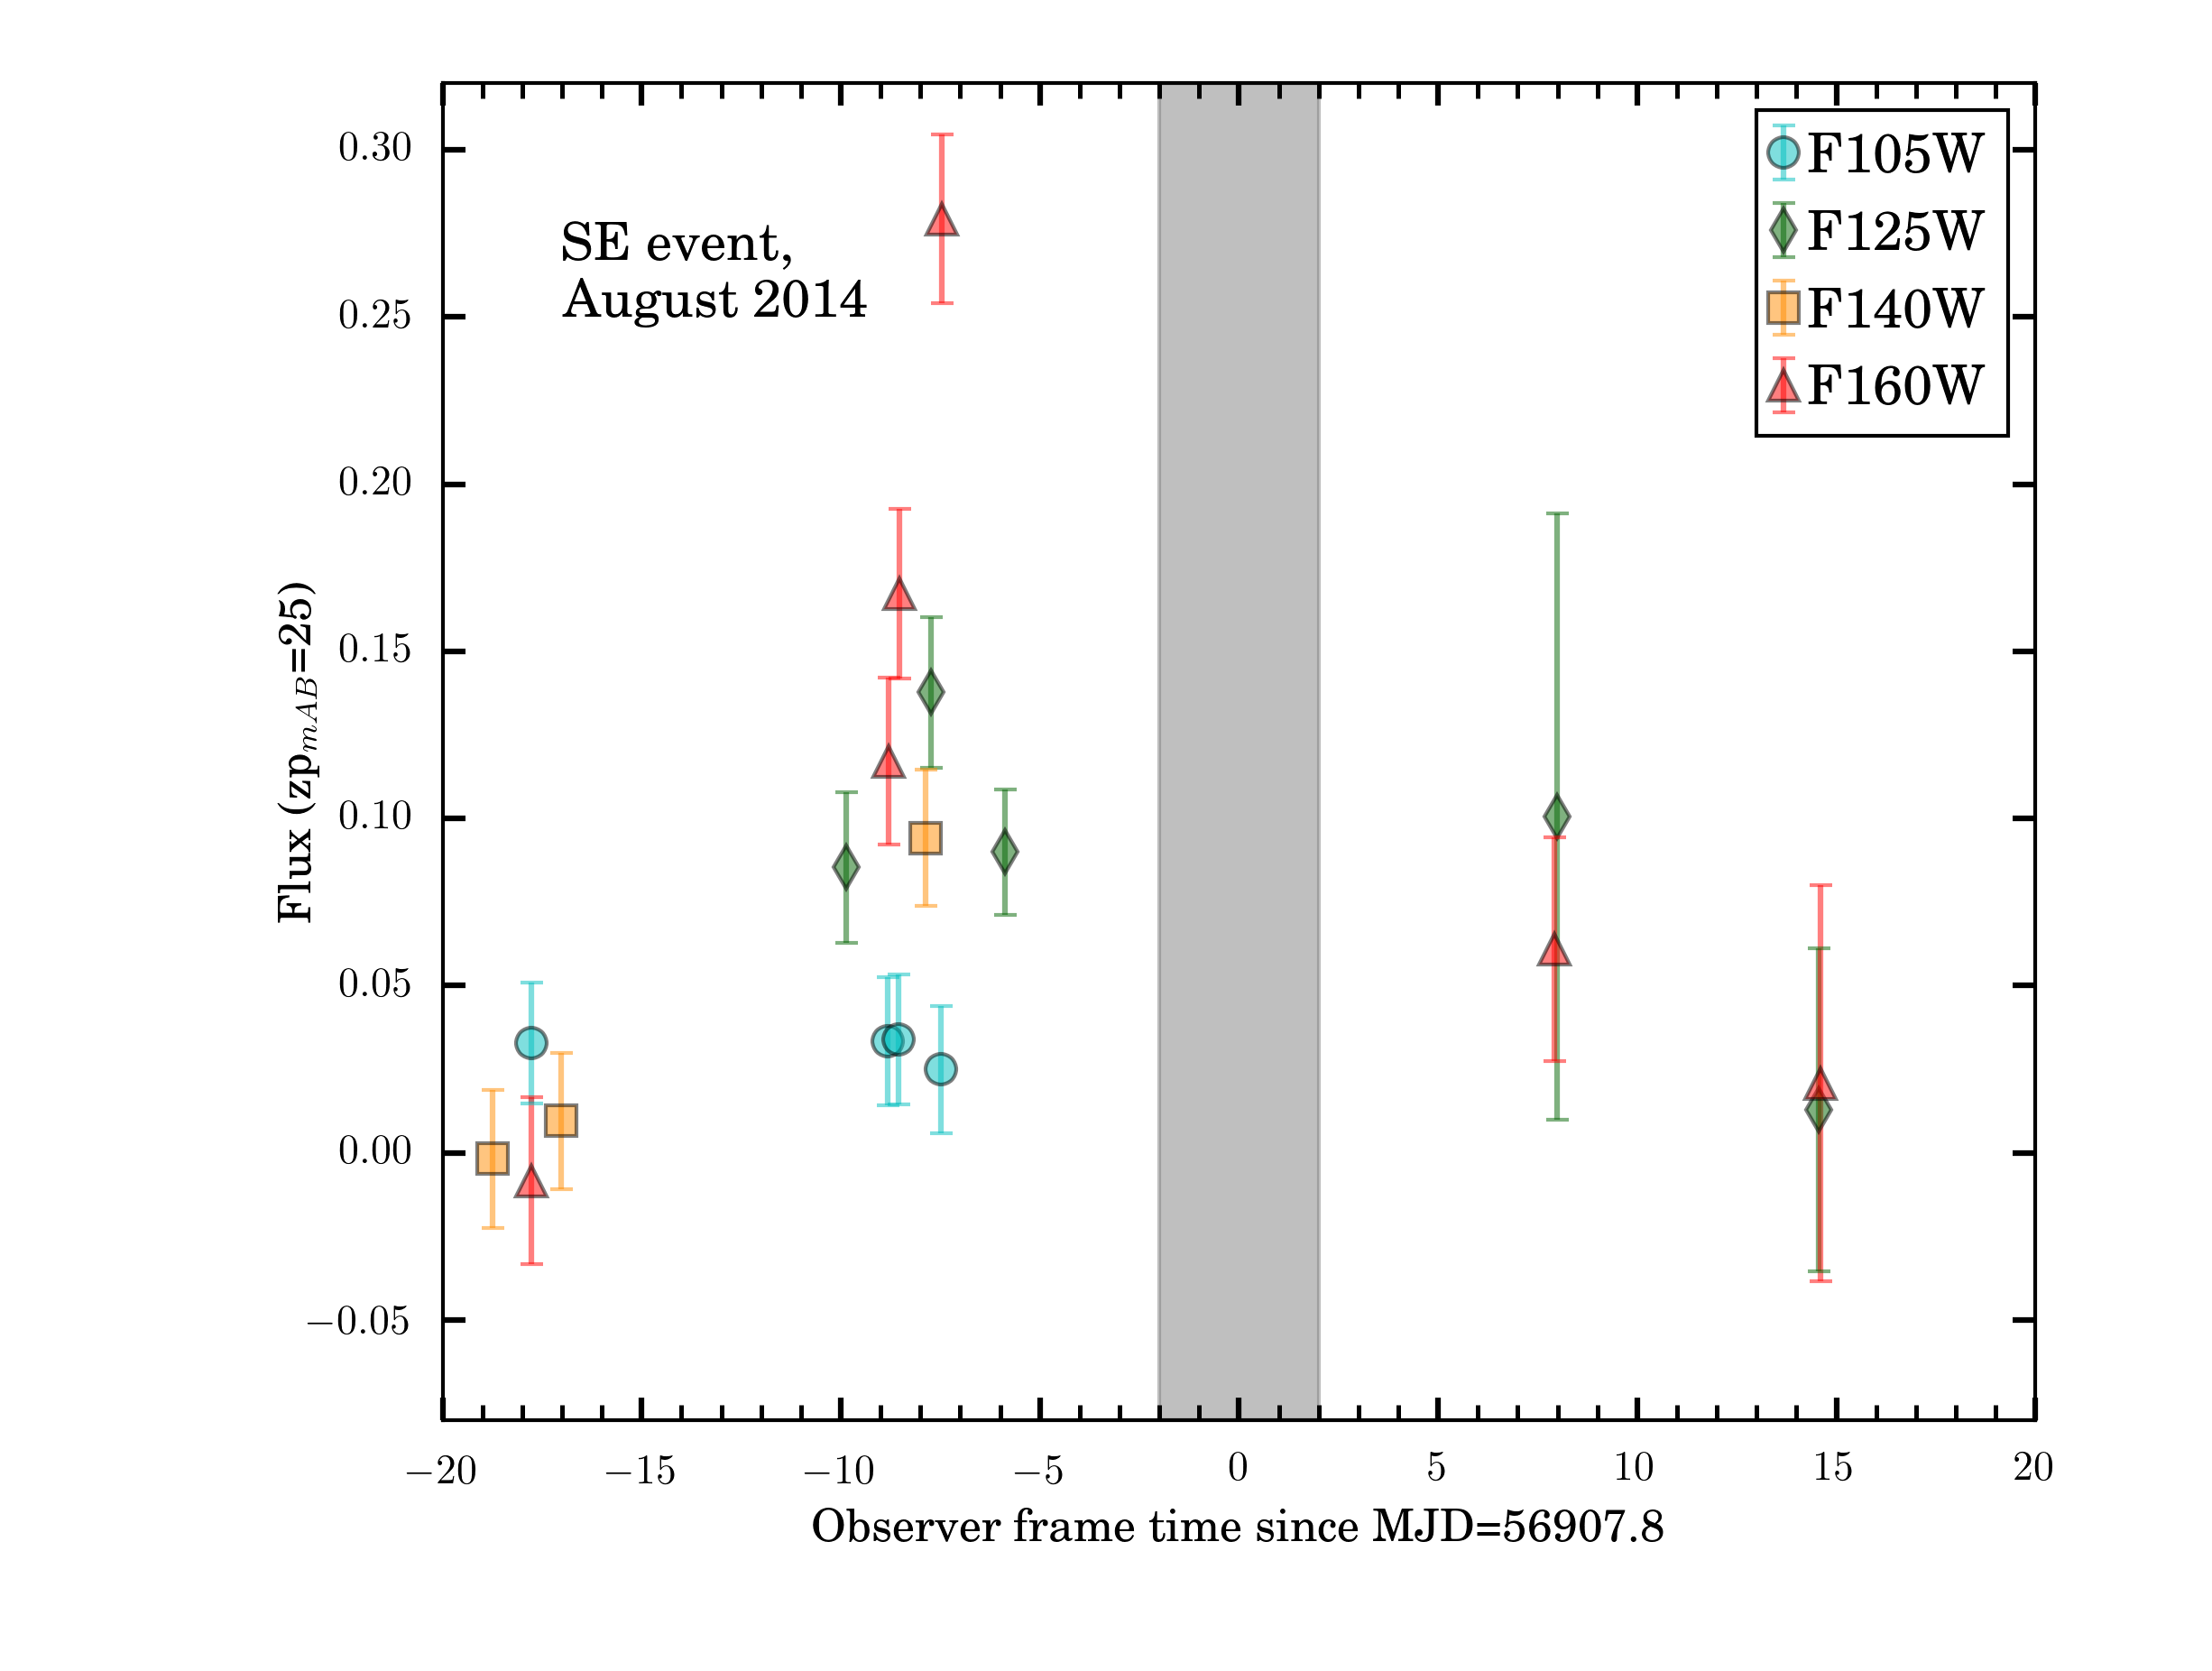
\includegraphics[width=\columnwidth]{figures/m0416_transient_SE.png}
\caption{The light curve of the January 2014 transient event, HFF14Spo-SE.}
\end{center}
\end{figure}

\begin{figure}
\begin{center}
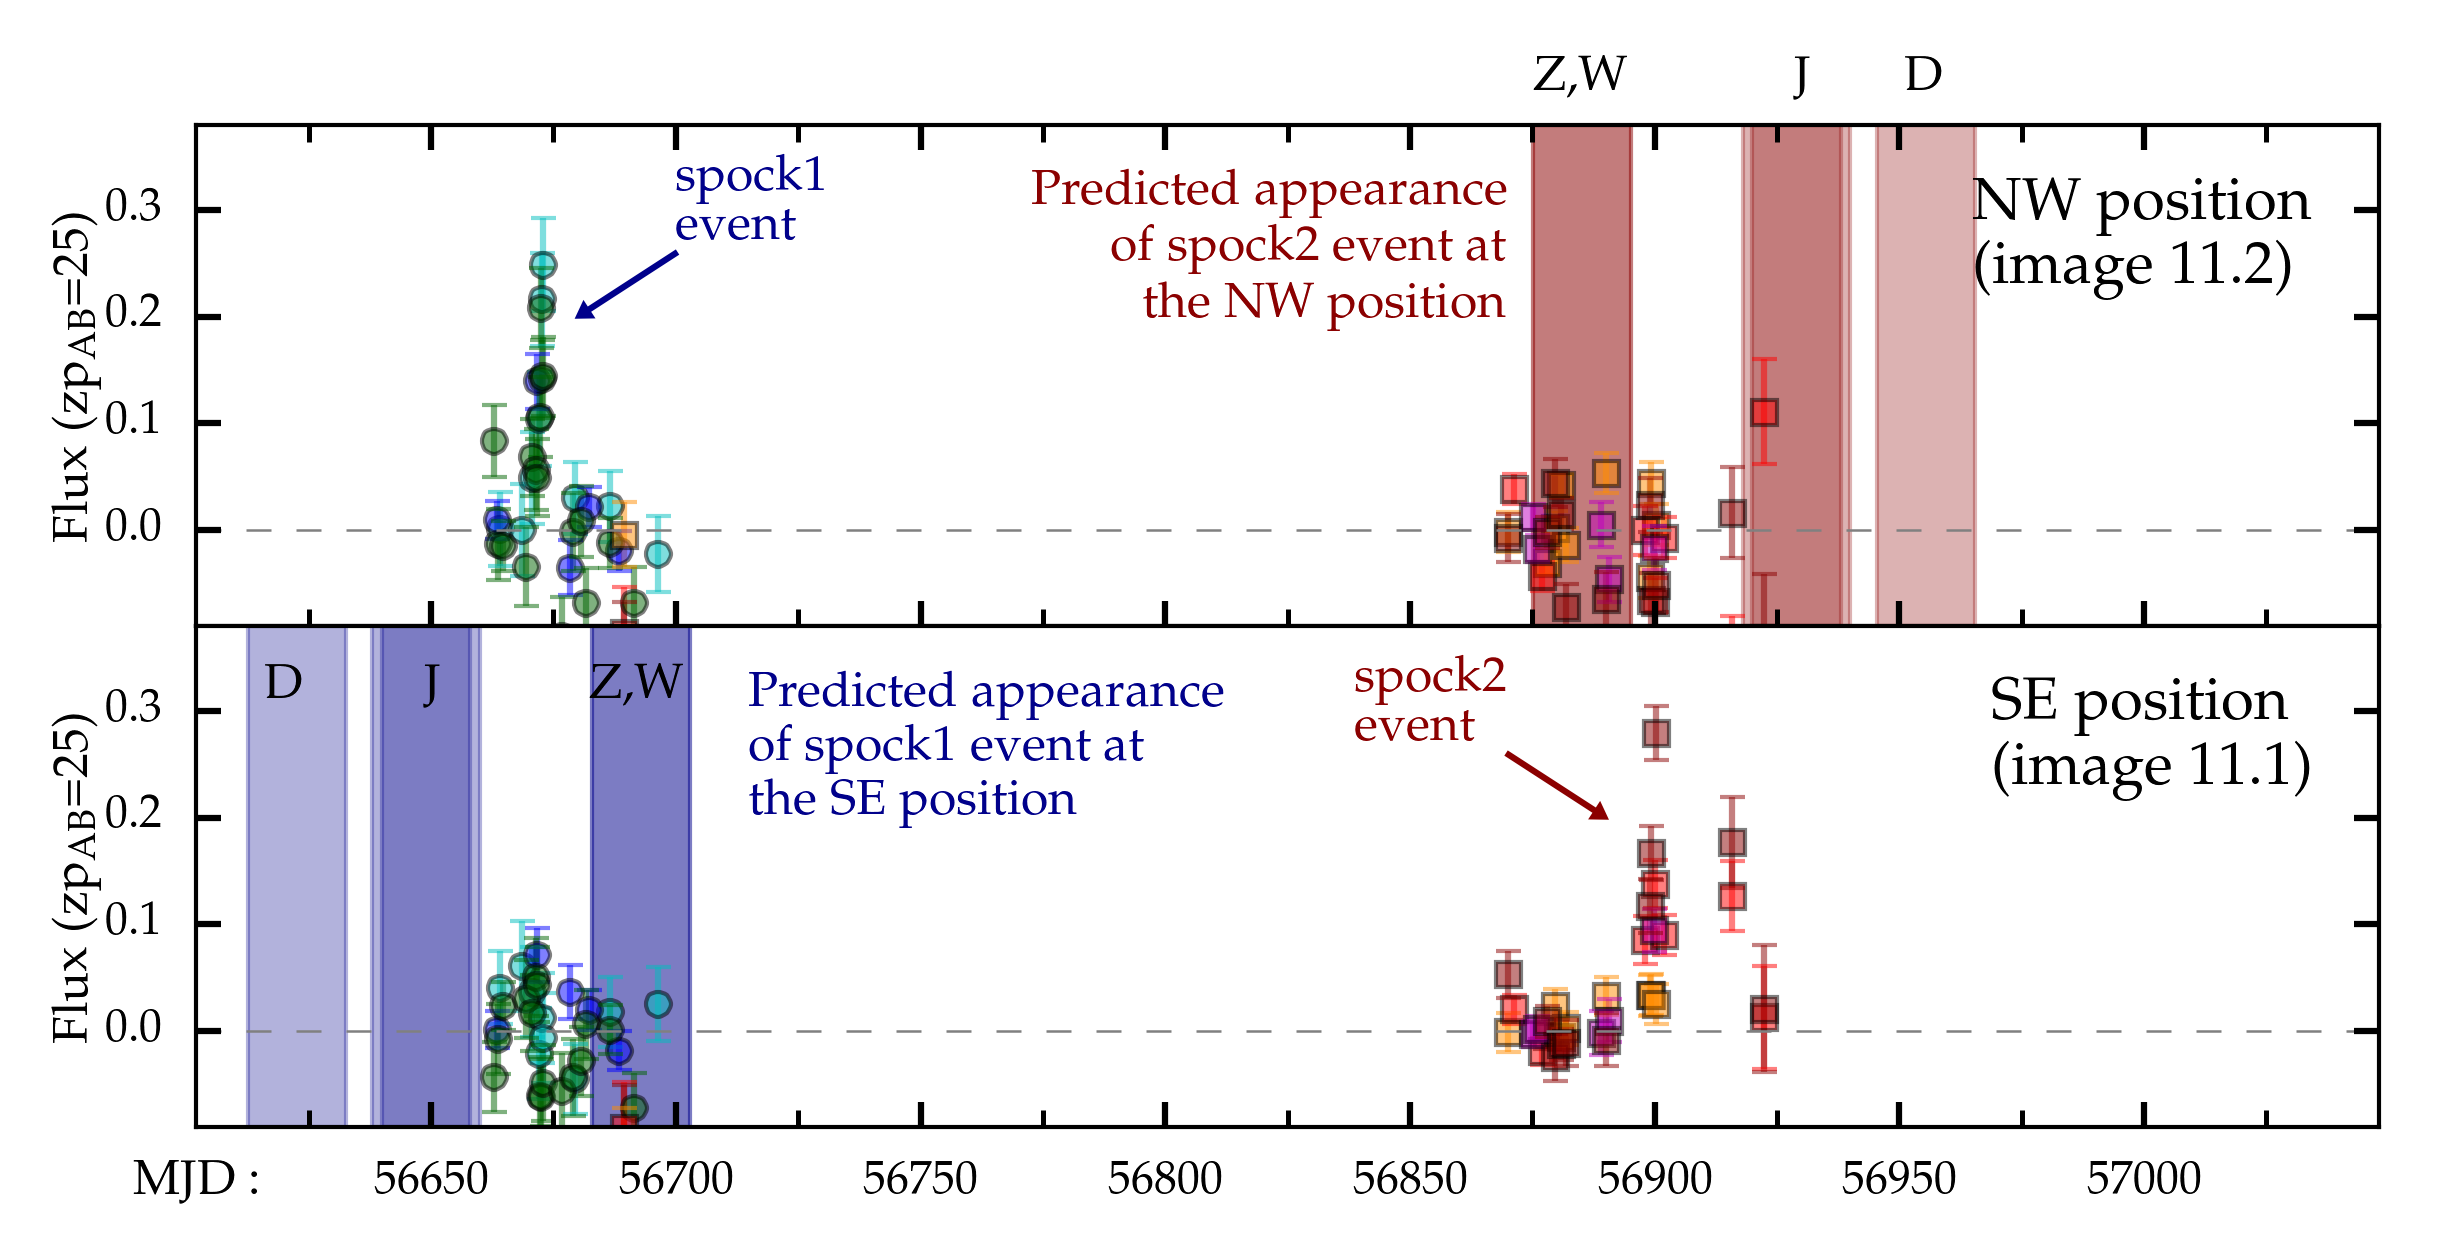
\includegraphics[width=\columnwidth]{figures/spock_predictions.png}
\caption{Lens model predictions for gravitational lensing time delays for both of the HFF14Spo events.}
\end{center}
\end{figure}


\section{Lens Models}\label{sec:LensModels}



  
  
  
  
  
